\documentclass[11pt]{article}
\usepackage{graphicx}

\title{Homework 05}
\author{Zach Stecher}
\date{Due: 11/15/16}

\begin{document}

\maketitle

\section*{Problem 1) Use k-means for a color clustering experiment on a portrait image of yourself.}

\subsection*{i. What happens when you increase or decrease the value of \textbf{n\_colors?}}

Reducing the value of \textbf{n\_colors} resulted in less options for classification, in turn resulting in less colors on the final image. The lower the number, the lower the amount of colors on the final image. The foreground image begins blending into the background.

\subsection*{ii. In what other possible applications do you think this can be useful?}

Color clustering seems like it could be useful for a number of recognition applications, or anything that requires separating a foreground image from a background. Facial recognition jumps out immediately. It might possibly be of use in medical imaging as well, to more easily separate out sections of interest from those that are normal.

\subsection*{iii. Why do you think the resulting picture was funny at the end?}

Lowering the value of \textbf{n\_colors} reduces the amount of colors the final image has access to. A normal image makes use of dozens of different colors(or more). Reducing the value down to as low as 2 results in the picture appropriating colors of nearby objects in the image to fill in the foreground portrait in order to best portray the original image with the new restrictions. The picture would probably end up looking funnier depending on what colors and the arrangement of them in the original image.

\section*{Problem 2) Run the provided python program and record your results.}

\subsection*{(c) Run the program for 1,000 samples and take note of the best number of neurons and eta.}
Results:

\begin{itemize}
\item Neurons 1, eta 0.1. Testing set CV score: -15.030426
\item Neurons 1, eta 0.2. Testing set CV score: -7.782941
\item Neurons 1, eta 0.7. Testing set CV score: -5.327886
\item Neurons 10, eta 0.2. Testing set CV score: -4.005331
\item Neurons 20, eta 0.3. Testing set CV score: -3.992921
\item Neurons 26, eta 0.2. Testing set CV score: -3.521599
\item Neurons 70, eta 0.1. Testing set CV score: -2.497174
\item Neurons 92, eta 0.1. Testing set CV score: -2.465212
\end{itemize}

From looking at these results, it seems that for a neural network to funtion optimally there must be a balance struck between the number of neurons used and the learning rate. While increasing the number of neurons seems to corrolate with increased accuracy on the surface, it seems like this can quickly turn into a problem of overfitting if not careful. 

\subsection*{(e) Run the program again for 10,000 samples. Note the difference.}

\begin{itemize}
\item Neurons 1, eta 0.1. Testing set CV score: -1.133346
\item Neurons 83, eta 0.1. Testing set CV score: -0.962296
\end{itemize}

These results were surprising to me when compared to the results from the previous experiment. I was expecting this experiment to yield more accurate results because of the increase in data points, but I did not expect for it to do so immediately. Right at 1 neuron this experiment achieved a CV score over 1.3 better than the best CV score for 1,000 data points. I was also surprised to see that it did not improve at all until 83 neurons, and only that one time. Based on the results from both of these experiments, the model's performance seems to peak somewhere near the middle-end of the amount of neurons we test. Since we only tested 1-100, I can't be sure that we have the optimal number of neurons out of all universal possibilities, but it seems that at a certain point the increase in neurons becomes not worth it for the trade-off in computational resources needed as well as the risk of overfitting the training data.

\begin{figure}[!htb]
\centering
	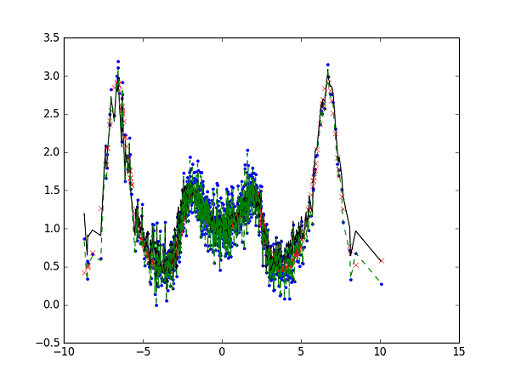
\includegraphics{NeuronGraph.png}
	\caption{Plot for 1,000 samples}
\end{figure}

\begin{figure}[!htb]
\centering
	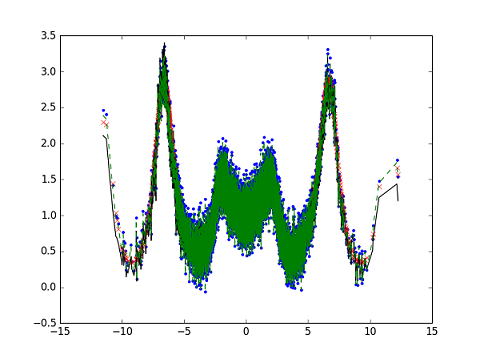
\includegraphics{NeuronGraph2.png}
	\caption{Plot for 10,000 samples}
\end{figure}

\end{document}